\documentclass[a4paper]{article}
\usepackage[utf8]{inputenc}
\usepackage[T1]{fontenc}
\usepackage[cache=false]{minted}
\usepackage[dvipsnames]{xcolor}
\usepackage{a4wide,syntax,listings,appendix,tikz,wrapfig,graphicx,hyperref}
\usepackage[margin=0.8in]{geometry}
\usepackage{pgfplots}
\usepackage{appendix}
\hypersetup{pdftitle={g08report},
pdfauthor={Pedro Mendes},
colorlinks=true,
urlcolor=blue,
linkcolor=black}
%\usetikzlibrary{arrows,positioning,automata,decorations.markings,shadows,shapes,calc}

\begin{document}

\title{Recomender System}
\author{Pedro Mendes (97144), Filipe Lucas (78775), Ricardo Pereira (86506)}
\date{\today}
\maketitle
%\tableofcontents

\section{Data Structure}
There were multiple approaches to store matrix A, the most basic one was
storing the values in a full matrix however as matrix A is sparse
we opted to store it as compressed sparse row (CSR) matrix. A CSR only stores
non-zero values in a single array making this a good choice in terms of
caching since all the values are stored in adjacent memory positions.

The other matrices were left as full matrices since they needed to be indexed in
$O(1)$ time and a CSR does not permit this.

\section{Matrix B multiplication}
A new matrix B needs to be calculated in every iteration, however, since the only
positions of matrix B that are needed in each iteration are the ones that
coincide with the non zero elements of matrix A, we optimized the code such that
only these positions are calculated.

Since the full matrix B is needed for the final output, after the iterations are
done the full matrix B is calculated.

\section{Solution}

The approach we took for parallelization was quite methodical. First we opted to
optimize the sequential version as far as we could. We experimented with using
\textit{openMP} in the inner loops but it always made the program very slow, even slower
than the sequential version.

\subsection{Matrix B}

As mentioned before there are two versions of the calculation. The simplest one
is the \texttt{full} one. Where each thread gets a distinct row and therefore
there are no race conditions possible.
\begin{minted}{c}
#pragma omp parallel for
for (size_t i = 0; i < l->rows; i++)
    for (size_t j = 0; j < r->columns; ++j)
        for (size_t k = 0; k < l->columns; ++k)
            // only write to shared memory: two threads never have the same i
            *MATRIX_AT(b, i, j) += *MATRIX_AT(l, i, k) * *MATRIX_AT(r, k, j);
\end{minted}

For the second version of we also have guarantees of no data races because each
thread gets a chunk of the indexes of A that do not overlap.
\begin{minted}{c}
Item const* const end = a->items + a->current_items;
#pragma omp parallel for
for (Item const* iter = a->items; iter < end; ++iter)
    double bij = 0.0;
    for (size_t k = 0; k < l->columns; k++)
        bij += *MATRIX_AT(l, iter->row, k) * *MATRIX_AT(r, k, iter->column);
    // only write to shared memory: two threads never have the same iter->row
    *MATRIX_AT(matrix, iter->row, iter->column) = bij;
\end{minted}

\subsection{Matrix R}

The calculation of matrix R was the easiest to parallelize, since, from the
sequential version, the top level for loop was over the rows of R we could
distribute theses rows over the threads and since the only write to shared
memory happens to R in distinct rows we have the guarantee that there are no
race conditions.

\begin{minted}{c}
#pragma omp parallel for
for (size_t k = 0; k < r->rows; k++)
    Item const* iter = // ...
    Item const* const end = // ...
    for (size_t column = 0; column < r->columns; column++)
        double aux = // sum of deltas of this column of A
        // only write to shared memory: two threads never have the same k
        *MATRIX_AT(aux_r, k, column) =
            *MATRIX_AT(r, k, column) - alpha * aux;
\end{minted}

\subsection{Matrix L}

Matrix L was also simple to parallelize once we figured out how to split the
rows of A between the threads. The outer loop is over the non empty rows of A
so we had to change this to be over all the possible rows of A, empty or not.
This would mean a loss of performance for the sequential version but it was
needed in order to split sets of rows between the threads. What this translates
to is a while loop that makes sure the A iterator is synchronized with the outer
loop.

In terms of race conditions the same reasoning applies. The only write to shared
memory depends on a variable that is private to each thread.

\begin{minted}{c}
Item const* iter = a->items;
Item const* const end = iter + a->current_items;
#pragma omp parallel for firstprivate(iter) schedule(guided)
for (size_t row = 0; row < a->n_rows; ++row)
    size_t row_len = a->row_lengths[row];
    while (iter != end && iter->row < row) iter += a->row_lengths[iter->row];
    for (size_t k = 0; k < l->columns; k++)
        double aux = // sum of deltas for this row of a
        // only write to shared memory: two threads never have the same row
        *MATRIX_AT(aux_l, row, k) = *MATRIX_AT(l, row, k) - alpha * aux;
    iter += row_len;
\end{minted}

\section{Speed up}
Disregarding the small instances, the speed up obtained, using 4 physical cores,
was close to 3x the serial version. Sometimes even reaching 3.5 times speed up
on some instances.

As for the scheduling, using guided brought a better speed up in some cases, but
also made some instances slower. The difference, however, was negligible.

The instances where guided was slightly better were the ones where the number of
non zero elements in matrix A were not evenly distributed between rows, so we
attribute the minimal difference to the fact that this unbalance of was also
minimal in all instances.

For these reasons we decided it was best to keep the guided version as it is more
resilient to possible unbalanced instances without incurring a significant cost
to the balanced ones.

\begin{figure}[H]
    \centering
        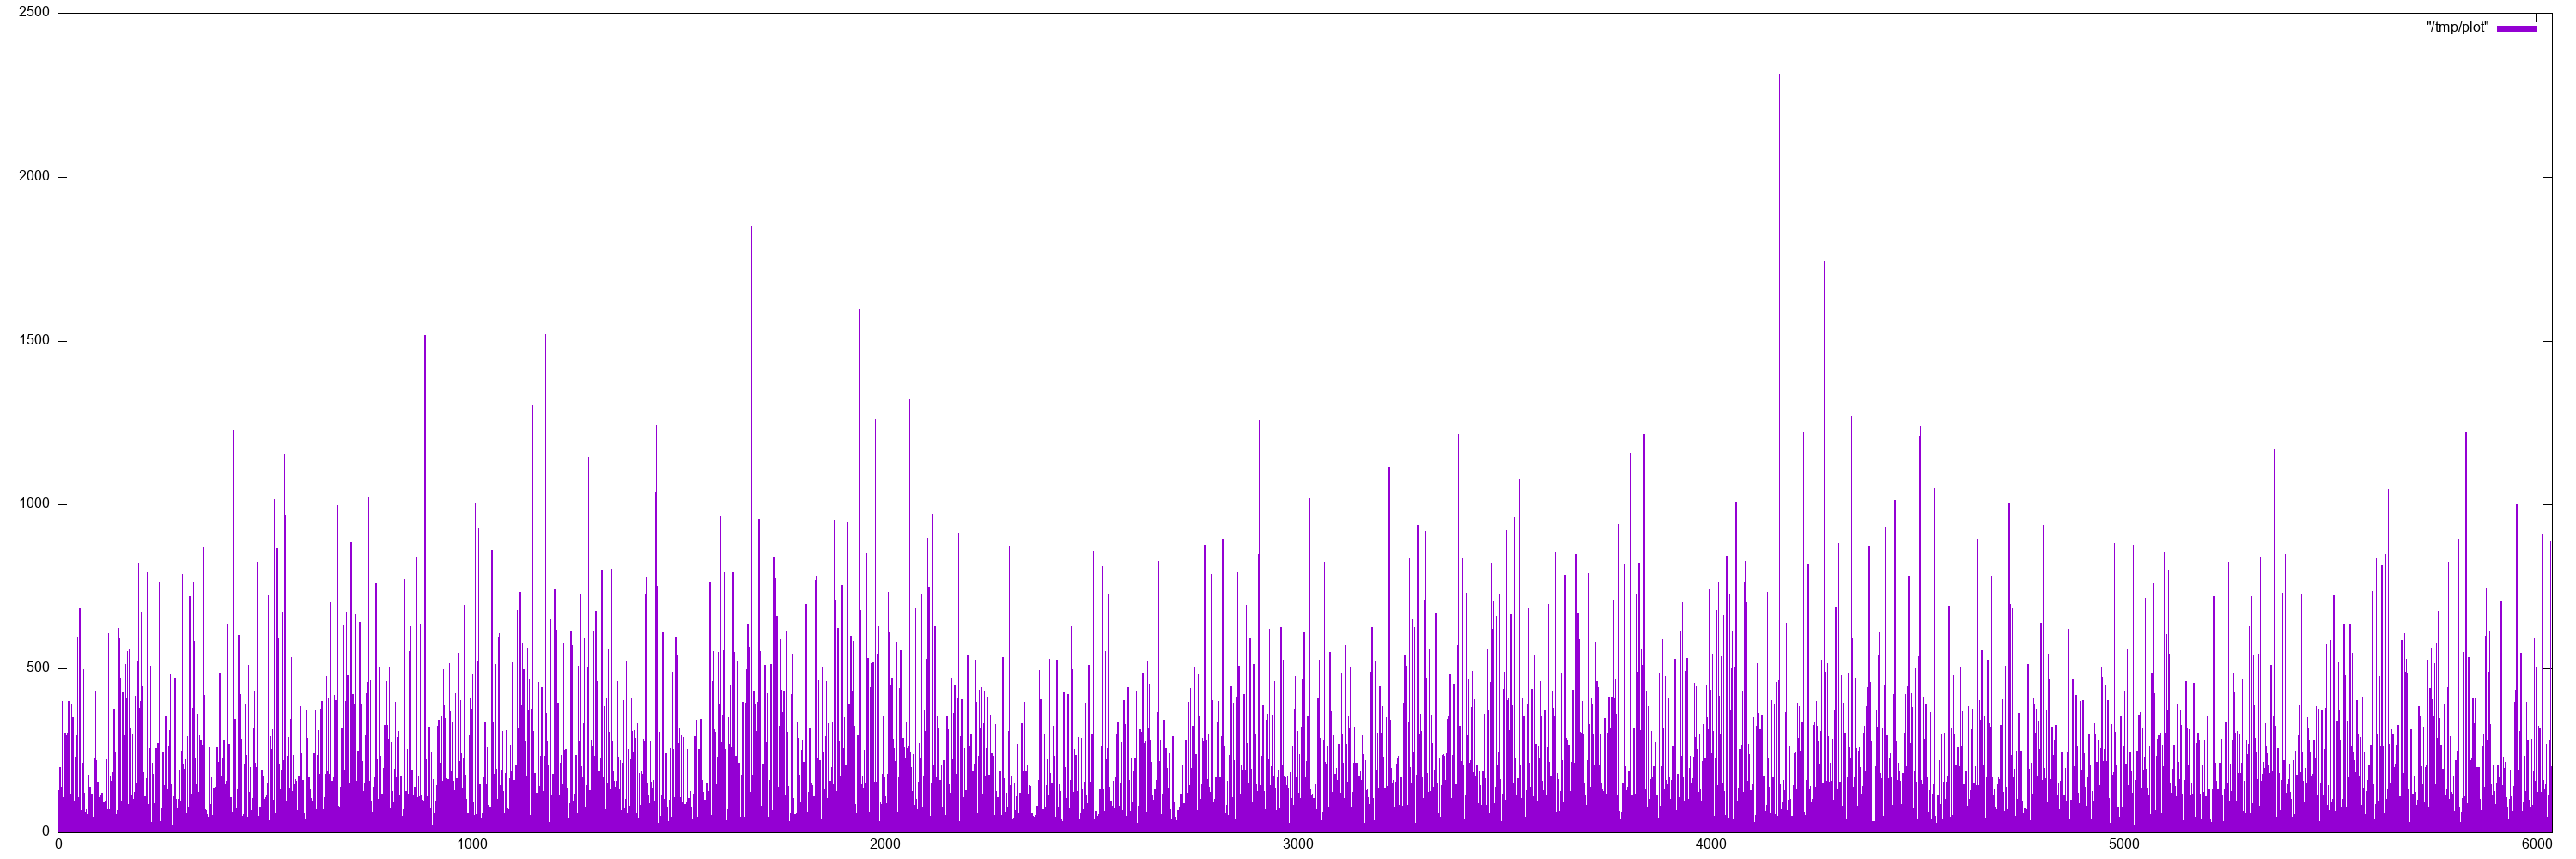
\includegraphics[width=\textwidth]{./ML1M.png}
        \caption{Number of non zero elements in each row of Matrix A.
        Example where some imbalance can be seen.}
\end{figure}


It is also important to note that, in bigger instances, the parsing creates a
significant overhead, making the speed up less noticeable.

\section{A note on hyper threading}

As can be seen in Appendix~\ref{app:bench} enabling hyper threading on 4 physical
cores has an interesting effect. When compared with the version with 4 threads
it brings little to no benefit, but when compared to forcing 8 threads on 4
physical cores it does improve the performance.

Sorted from best to worse:

\begin{itemize}
    \item 8 threads on 4 hyper threaded cores;
    \item 4 threads on 4 cores;
    \item 8 threads on 4 cores;
\end{itemize}


\section{Future Work}
In a future implementation the parser could be made parallel to see if could
bring further improvements. This seems unlikely as the chunks of the parsed
input need to be aggregated at the end of the parsing and this could prove to be
too much to compensate the overhead it might bring to smaller instances.

\pagebreak
\begin{appendices}
    \section{Benchmarks}\label{app:bench}
    These benchmarks were run on an Intel i5-8250U @ 3.400GHz with 4 physical
    cores with hyper threading disabled as to not interfere with the
    measurements. The last graph shows the results with hyper threading enabled
    for comparison.

    \subsection{Number of threads equal to 1}

    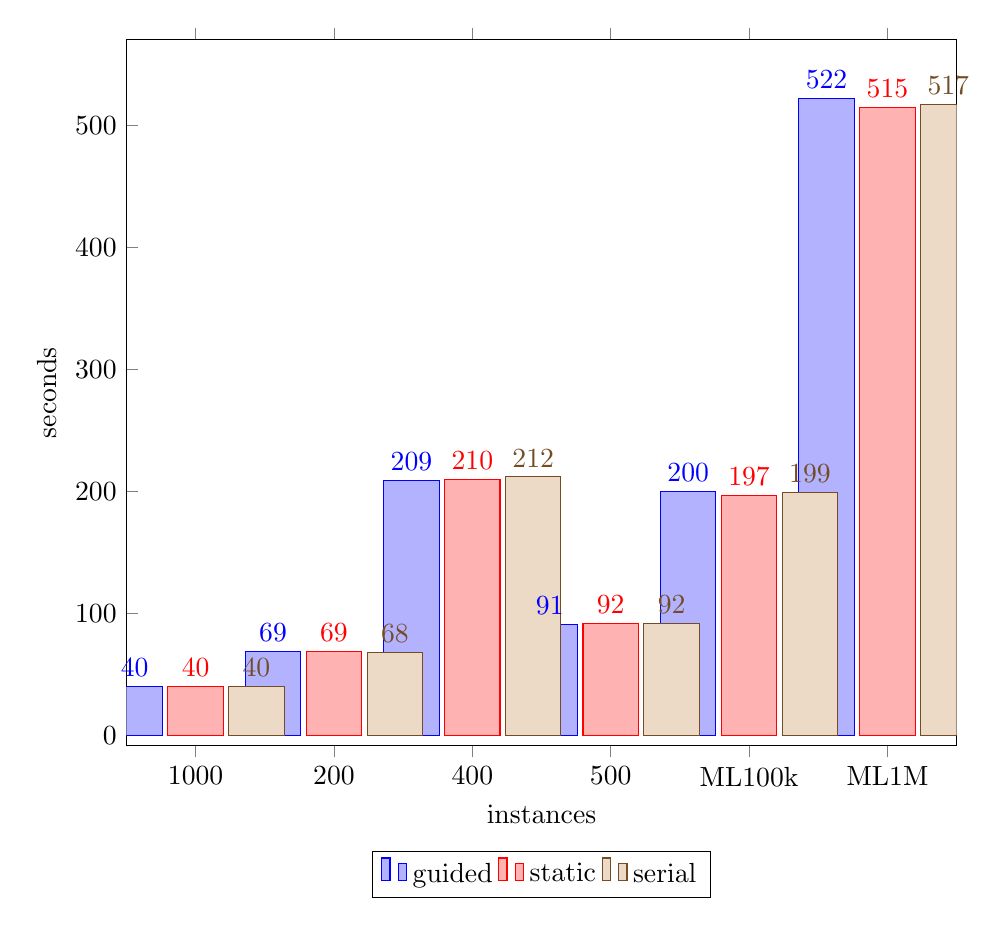
\begin{tikzpicture}
    \begin{axis}[
            ybar,
            enlargelimits=true,
            bar width=20pt,
            width=\textwidth,
            height=300pt,
            legend style={at={(0.5,-0.15)}, anchor=north,legend columns=-1},
            ylabel={seconds},
            xlabel={instances},
            symbolic x coords={1000,200,400,500,ML100k,ML1M},
            xtick=data,
            nodes near coords,
            nodes near coords align={vertical},
        ]
\addplot coordinates {
(1000,40)	% ./guided_new_parser_bin
(200,69)	% ./guided_new_parser_bin
(400,209)	% ./guided_new_parser_bin
(500,91)	% ./guided_new_parser_bin
(ML100k,200)	% ./guided_new_parser_bin
(ML1M,522)	% ./guided_new_parser_bin
};
\addplot coordinates {
(1000,40)	% ./static_new_parser_bin
(200,69)	% ./static_new_parser_bin
(400,210)	% ./static_new_parser_bin
(500,92)	% ./static_new_parser_bin
(ML100k,197)	% ./static_new_parser_bin
(ML1M,515)	% ./static_new_parser_bin
};
\addplot coordinates {
(1000,40)	% ./serial_new_parser_bin
(200,68)	% ./serial_new_parser_bin
(400,212)	% ./serial_new_parser_bin
(500,92)	% ./serial_new_parser_bin
(ML100k,199)	% ./serial_new_parser_bin
(ML1M,517)	% ./serial_new_parser_bin
};

        \legend{guided, static, serial}
    \end{axis}
\end{tikzpicture}
}

    \subsection{Number of threads equal to 2}

    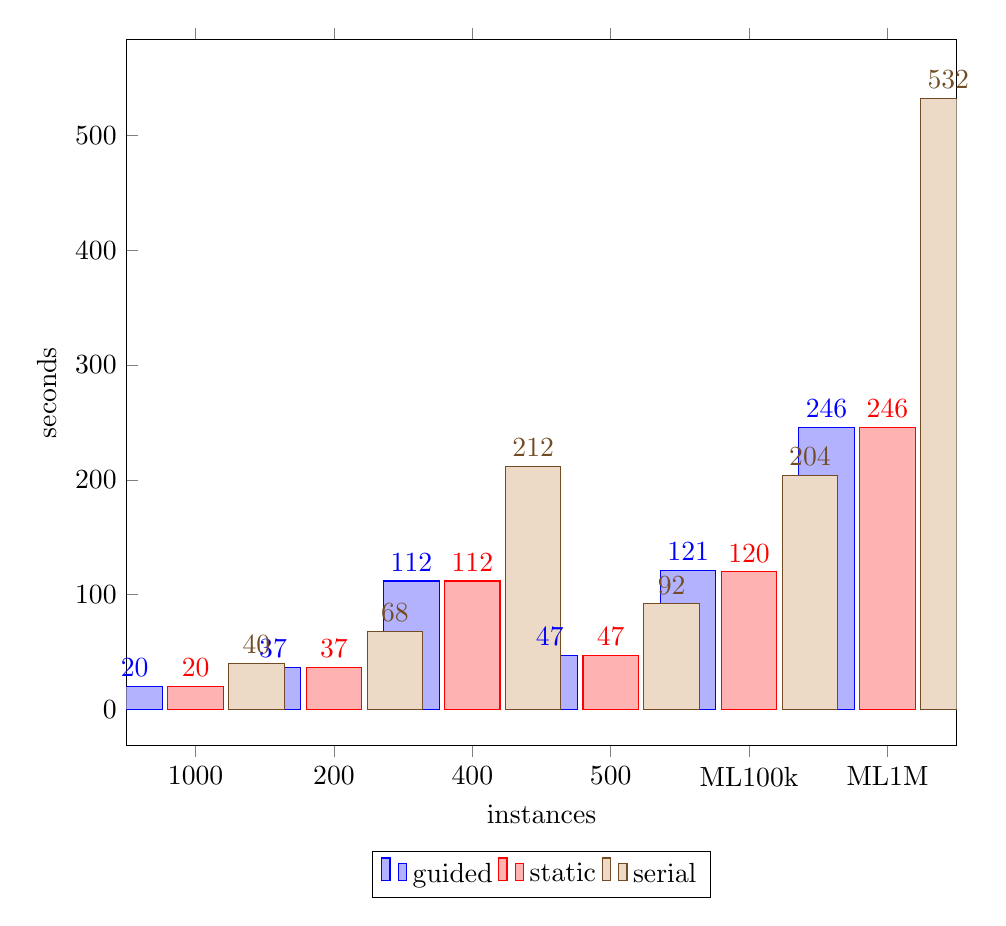
\begin{tikzpicture}
    \begin{axis}[
            ybar,
            enlargelimits=true,
            bar width=20pt,
            width=\textwidth,
            height=300pt,
            legend style={at={(0.5,-0.15)}, anchor=north,legend columns=-1},
            ylabel={seconds},
            xlabel={instances},
            symbolic x coords={1000,200,400,500,ML100k,ML1M},
            xtick=data,
            nodes near coords,
            nodes near coords align={vertical},
        ]
\addplot coordinates {
(1000,20)	% ./guided_new_parser_bin
(200,37)	% ./guided_new_parser_bin
(400,112)	% ./guided_new_parser_bin
(500,47)	% ./guided_new_parser_bin
(ML100k,121)	% ./guided_new_parser_bin
(ML1M,246)	% ./guided_new_parser_bin
};
\addplot coordinates {
(1000,20)	% ./static_new_parser_bin
(200,37)	% ./static_new_parser_bin
(400,112)	% ./static_new_parser_bin
(500,47)	% ./static_new_parser_bin
(ML100k,120)	% ./static_new_parser_bin
(ML1M,246)	% ./static_new_parser_bin
};
\addplot coordinates {
(1000,40)	% ./serial_new_parser_bin
(200,68)	% ./serial_new_parser_bin
(400,212)	% ./serial_new_parser_bin
(500,92)	% ./serial_new_parser_bin
(ML100k,204)	% ./serial_new_parser_bin
(ML1M,532)	% ./serial_new_parser_bin
};

        \legend{guided, static, serial}
    \end{axis}
\end{tikzpicture}
}

    \subsection{Number of threads equal to 4}

    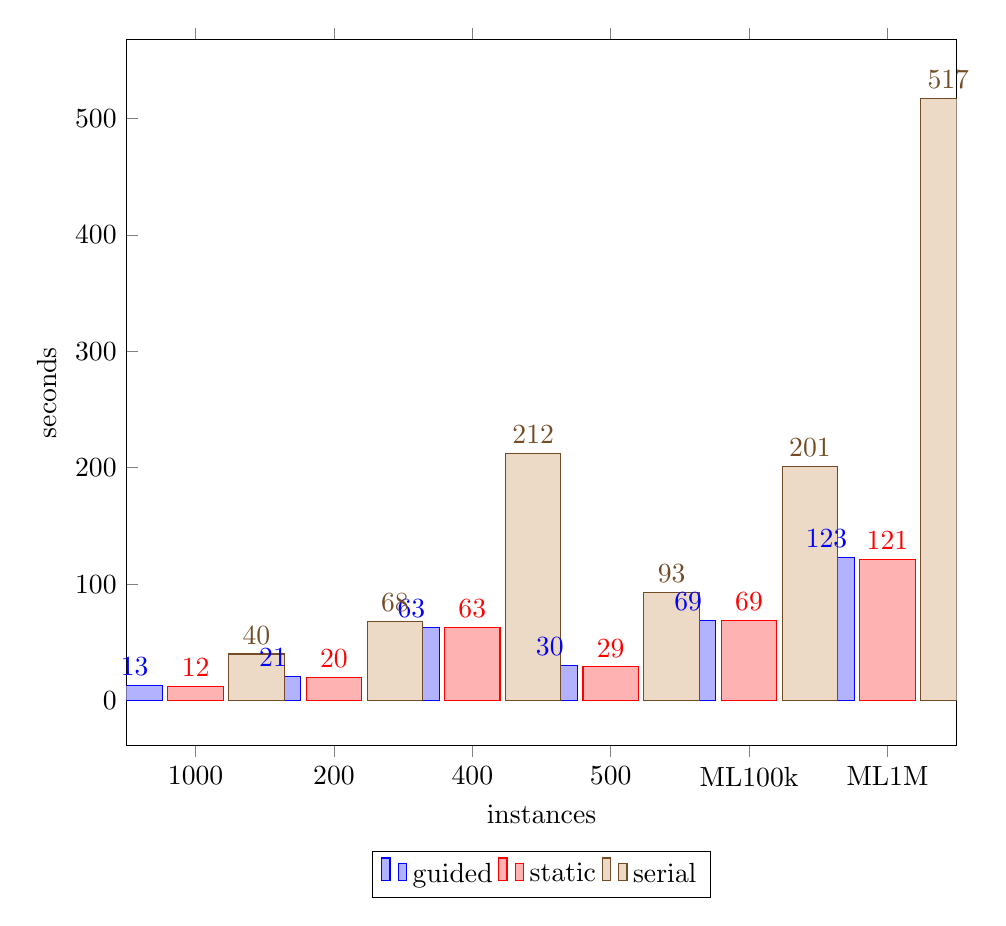
\begin{tikzpicture}
    \begin{axis}[
            ybar,
            enlargelimits=true,
            bar width=20pt,
            width=\textwidth,
            height=300pt,
            legend style={at={(0.5,-0.15)}, anchor=north,legend columns=-1},
            ylabel={seconds},
            xlabel={instances},
            symbolic x coords={1000,200,400,500,ML100k,ML1M},
            xtick=data,
            nodes near coords,
            nodes near coords align={vertical},
        ]
\addplot coordinates {
(1000,13)	% ./guided_new_parser_bin
(200,21)	% ./guided_new_parser_bin
(400,63)	% ./guided_new_parser_bin
(500,30)	% ./guided_new_parser_bin
(ML100k,69)	% ./guided_new_parser_bin
(ML1M,123)	% ./guided_new_parser_bin
};
\addplot coordinates {
(1000,12)	% ./static_new_parser_bin
(200,20)	% ./static_new_parser_bin
(400,63)	% ./static_new_parser_bin
(500,29)	% ./static_new_parser_bin
(ML100k,69)	% ./static_new_parser_bin
(ML1M,121)	% ./static_new_parser_bin
};
\addplot coordinates {
(1000,40)	% ./serial_new_parser_bin
(200,68)	% ./serial_new_parser_bin
(400,212)	% ./serial_new_parser_bin
(500,93)	% ./serial_new_parser_bin
(ML100k,201)	% ./serial_new_parser_bin
(ML1M,517)	% ./serial_new_parser_bin
};

        \legend{guided, static, serial}
    \end{axis}
\end{tikzpicture}
}

    \subsection{Number of threads equal to 8}

    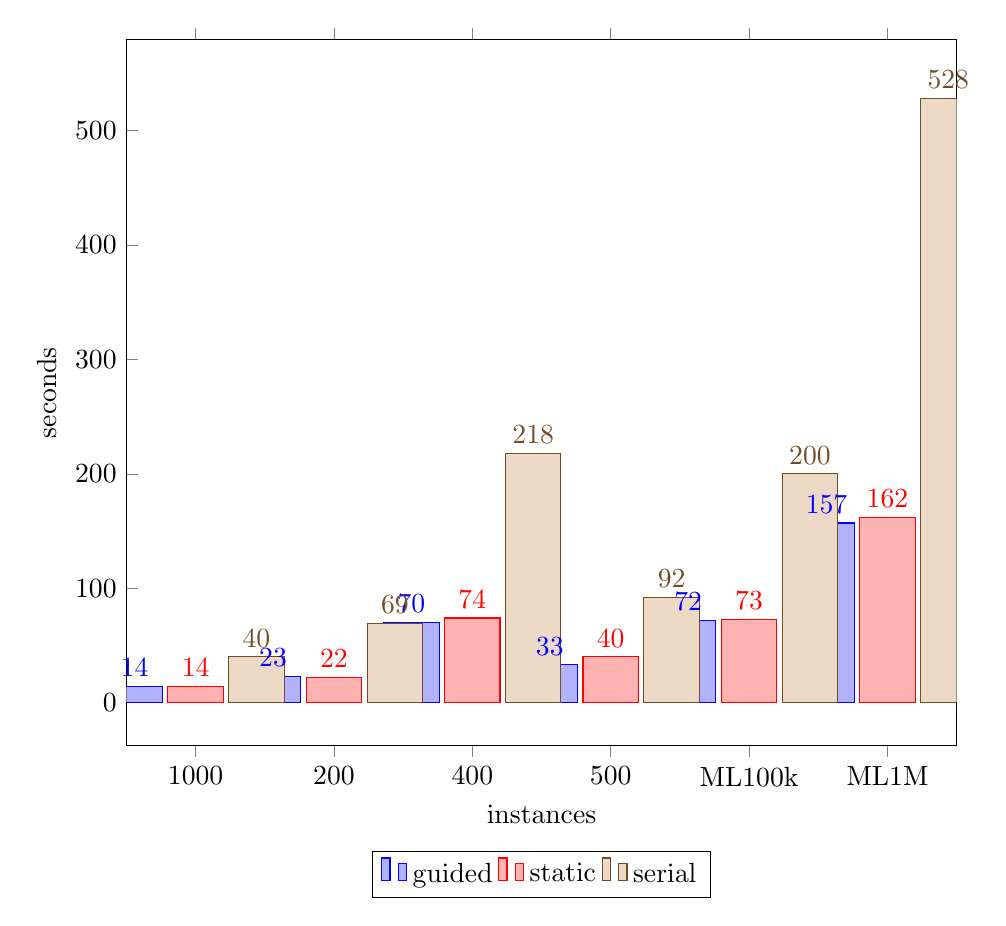
\begin{tikzpicture}
    \begin{axis}[
            ybar,
            enlargelimits=true,
            bar width=20pt,
            width=\textwidth,
            height=300pt,
            legend style={at={(0.5,-0.15)}, anchor=north,legend columns=-1},
            ylabel={seconds},
            xlabel={instances},
            symbolic x coords={1000,200,400,500,ML100k,ML1M},
            xtick=data,
            nodes near coords,
            nodes near coords align={vertical},
        ]
\addplot coordinates {
(1000,14)	% ./guided_new_parser_bin
(200,23)	% ./guided_new_parser_bin
(400,70)	% ./guided_new_parser_bin
(500,33)	% ./guided_new_parser_bin
(ML100k,72)	% ./guided_new_parser_bin
(ML1M,157)	% ./guided_new_parser_bin
};
\addplot coordinates {
(1000,14)	% ./static_new_parser_bin
(200,22)	% ./static_new_parser_bin
(400,74)	% ./static_new_parser_bin
(500,40)	% ./static_new_parser_bin
(ML100k,73)	% ./static_new_parser_bin
(ML1M,162)	% ./static_new_parser_bin
};
\addplot coordinates {
(1000,40)	% ./serial_new_parser_bin
(200,69)	% ./serial_new_parser_bin
(400,218)	% ./serial_new_parser_bin
(500,92)	% ./serial_new_parser_bin
(ML100k,200)	% ./serial_new_parser_bin
(ML1M,528)	% ./serial_new_parser_bin
};

        \legend{guided, static, serial}
    \end{axis}
\end{tikzpicture}
}

    \subsection{Number of threads equal to 8 with hyper threading}

    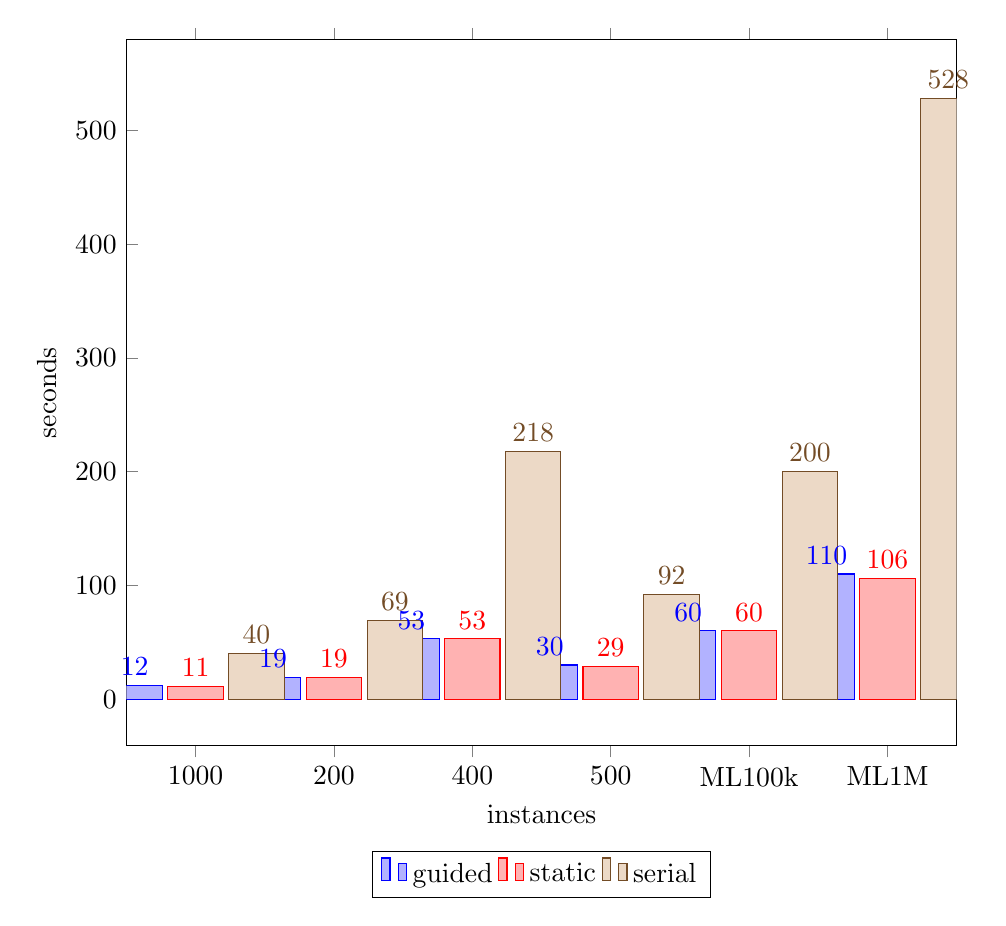
\begin{tikzpicture}
    \begin{axis}[
            ybar,
            enlargelimits=true,
            bar width=20pt,
            width=\textwidth,
            height=300pt,
            legend style={at={(0.5,-0.15)}, anchor=north,legend columns=-1},
            ylabel={seconds},
            xlabel={instances},
            symbolic x coords={1000,200,400,500,ML100k,ML1M},
            xtick=data,
            nodes near coords,
            nodes near coords align={vertical},
        ]
\addplot coordinates {
(1000,12)	% ./guided_new_parser_bin
(200,19)	% ./guided_new_parser_bin
(400,53)	% ./guided_new_parser_bin
(500,30)	% ./guided_new_parser_bin
(ML100k,60)	% ./guided_new_parser_bin
(ML1M,110)	% ./guided_new_parser_bin
};
\addplot coordinates {
(1000,11)	% ./static_new_parser_bin
(200,19)	% ./static_new_parser_bin
(400,53)	% ./static_new_parser_bin
(500,29)	% ./static_new_parser_bin
(ML100k,60)	% ./static_new_parser_bin
(ML1M,106)	% ./static_new_parser_bin
};
\addplot coordinates {
(1000,40)	% ./serial_new_parser_bin
(200,69)	% ./serial_new_parser_bin
(400,218)	% ./serial_new_parser_bin
(500,92)	% ./serial_new_parser_bin
(ML100k,200)	% ./serial_new_parser_bin
(ML1M,528)	% ./serial_new_parser_bin
};

        \legend{guided, static, serial}
    \end{axis}
\end{tikzpicture}
}
\end{appendices}

%ADD PRETTY GRAPHS!
%add tables
\end{document}

